%\documentclass[12pt,twoside]{extbook}
\documentclass[12pt,oneside]{extbook}
\usepackage[utf8]{inputenc}
\usepackage[spanish, mexico]{babel}
\usepackage[T1]{fontenc}
\usepackage[hidelinks,bookmarks=true,pdfpagelabels]{hyperref}

%%%%%%%%%%% Para edicion %%%%%%%%%%%%%%%
\usepackage{amsmath,latexsym,color,url}
\usepackage{epsfig,enumitem,appendix,authblk}
\usepackage{amsthm}
\usepackage{amssymb}
\usepackage{textcomp}
\usepackage{mathtools}
\usepackage{amstext}
\usepackage{units}
\usepackage{array}
\tolerance=1
\emergencystretch=\maxdimen
\hyphenpenalty=10000
\hbadness=10000
%%%%%%%%%%%%%%%%%%%%%%%%%%%%%%%%%%%%%%%%

%%%%%%%%% Para imagenes %%%%%%%%%%%%
\usepackage{graphicx}
\graphicspath{ {images/} }
\usepackage{caption}
\usepackage{subcaption}
%%%%%%%%%%%%%%%%%%%%%%%%%%%%%%%%%%%%%

%%%%%%%%%%%%%%%%%%%%%%% Page layout %%%%%%%%%%%%%%%%%%%%%
\usepackage[width=140mm,top=30mm,bottom=30mm,bindingoffset=6mm,paperwidth=20cm,paperheight=22.5cm]{geometry}
%\usepackage[width=150mm,top=25mm,bottom=25mm,bindingoffset=6mm,paperwidth=17cm,paperheight=22.5cm]{geometry}
%%%%%%%%%%%%%%%%%%%%%%%%%%%%%%%%%%%%%%%%%%%%%%%%%%%%%%%%%%

%%%%%%%%%%%%%% Delimitadores %%%%%%%%%%%%%%%%%%
\DeclarePairedDelimiter\ceil{\lceil}{\rceil}
\DeclarePairedDelimiter\floor{\lfloor}{\rfloor}
\newcommand*{\vertbar}{\rule[1ex]{0.5pt}{2.5ex}}
\newcommand*{\horzbar}{\rule[.5ex]{2.5ex}{0.5pt}}
\providecommand{\abs}[1]{\lvert#1\rvert}
\providecommand{\norm}[1]{\lVert#1\rVert}
\DeclareMathOperator{\gen}{gen}
\DeclareMathOperator{\rango}{rango}
\newcommand{\mcd}[1]{\operatorname{mcd}\left(#1\right)}
\newcommand{\Mod}[1]{\ (\text{mod}\ #1)}
\newcommand{\bigslant}[2]{{\left.\raisebox{.2em}{$#1$}\middle/\raisebox{-.2em}{$#2$}\right.}}
%%%%%%%%%%%%%%%%%%%%%%%%%%%%%%%%%%%%%%%%%%%%%%%

%%%%%%%%%%%%% Para bibliografía %%%%%%%%%%%%%%%
%Society for Industrial and Applied Mathematics
\usepackage[square,sort,comma,numbers]{natbib}
\bibliographystyle{siam}
%%%%%%%%%%%%%%%%%%%%%%%%%%%%%%%%%%%%%%%%%%%%%%%

%%%%%%%%%%%%%%%%% Para tablas %%%%%%%%%%%%%%%%%
\usepackage{tabularx}
%%%%%%%%%%%%%%%%%%%%%%%%%%%%%%%%%%%%%%%%%%%%%%%

%%%%%%%%%% Para listados de programas %%%%%%%%%
\usepackage{listings}
\usepackage{mdframed}
% \vspace{5mm}
% \lstset{frame=none}
% \begin{mdframed}
% \begin{centering}
% \begin{lstlisting}
% ...
% \end{lstlisting}
% \par\end{centering}
% \end{mdframed}
% \lstset{frame=b}
% \vspace{5mm}
%%%%%%%%%%%%%%%%%%%%%%%%%%%%%%%%%%%%%%%%%%%%%%%%

% Para codigo de Java, C++, R, Matlab, Python, etc %
% \lstinputlisting[label=et,caption={}]{archivo.R}
\usepackage{listings}
\usepackage{courier}
\usepackage{caption}
 \lstset{
         basicstyle=\footnotesize\ttfamily,
         numberstyle=\tiny,
         numbersep=5pt,
         tabsize=2,
         extendedchars=true,
         breaklines=true,
         keywordstyle=\color{red},
                frame=b,
         stringstyle=\color{white}\ttfamily,
         showspaces=false,
         showtabs=false,
         xleftmargin=17pt,
         framexleftmargin=17pt,
         framexrightmargin=5pt,
         framexbottommargin=4pt,
         showstringspaces=false
 }
\lstloadlanguages{R}%Java, C++, Python, R, Matlab...
\DeclareCaptionFont{white}{\color{white}}
\DeclareCaptionFormat{listing}{\colorbox[cmyk]{0.43, 0.35, 0.35,0.01}{\parbox{\textwidth}{\hspace{15pt}#1#2#3}}}
\captionsetup[lstlisting]{format=listing,labelfont=white,textfont=white, singlelinecheck=false, margin=0pt, font={bf,footnotesize}}
\renewcommand\lstlistingname{Código}
\newcommand{\HRule}{\rule{\linewidth}{0.5mm}}
\newcount\mycount
%%%%%%%%%%%%%%%%%%%%%%%%%%%%%%%%%%%%%%%%%%%%%%%%%%%

%%%%%%%%%%%%%%%%% Para algoritmos %%%%%%%%%%%%%%%%%
\usepackage[lined,boxed,linesnumbered]{algorithm2e}
\SetKwInput{Input}{Entrada}
\SetKwInput{Output}{Salida}
\SetKwIF{If}{ElseIf}{Else}{Si}{entonces}{De otro modo si}{De otro modo}{Fin}
\SetKwFor{For}{Para}{ }{Fin}
\SetKwFor{While}{Mientras}{ }{Fin}
\SetKwRepeat{Do}{Hacer}{Mientras}
\newenvironment{algoritmo}[1][htb]
  {\renewcommand{\algorithmcfname}{Algoritmo}
   \begin{algorithm}[#1]
  }{\end{algorithm}}
%%%%%%%%%%%%%%%%%%%%%%%%%%%%%%%%%%%%%%%%%%%%%%%%%%%

%%%%%%%%%%%%%%%%%%% Etiquetas %%%%%%%%%%%%%%%%%%%%%
\theoremstyle{plain}
\newtheorem{theorem}{Teorema}[chapter]
\newtheorem{lemma}[theorem]{Lema}
\newtheorem{proposition}[theorem]{Proposición}
\newtheorem{axiom}[theorem]{Axioma}
\newtheorem{case}[theorem]{Caso}
\newtheorem{conclusion}[theorem]{Conclusión}
\newtheorem{condition}[theorem]{Condición}
\newtheorem{conjecture}[theorem]{Conjetura}
\newtheorem{corollary}[theorem]{Corolario}
\newtheorem{criterion}[theorem]{Criterio}
\theoremstyle{definition}
\newtheorem{definition}[theorem]{Definición}
\newtheorem{example}[theorem]{Ejemplo}
\newtheorem{exercise}[theorem]{Ejercicio}
\newtheorem{notation}[theorem]{Notación}
\newtheorem{problem}[theorem]{Problema}
\newtheorem{remark}[theorem]{Comentario}
\newtheorem{solution}[theorem]{Solución}
\newtheorem{summary}[theorem]{Resumen}
\theoremstyle{remark}
\newtheorem*{rem}{Observación}
\newtheorem*{note}{Nota}
%%%%%%%%%%%%%%%%%%%%%%%%%%%%%%%%%%%%%%%%%%%%%%%%%%%


\title{Vector Error-Correction Model}
\author{Omar Díaz Landa}
\date{2016}

\begin{document}

\frontmatter
\begin{titlepage}
    \begin{center}
        
        \vspace{0.2cm}

        \large
        \textbf{INSTITUTO TECNOLÓGICO AUTÓNOMO DE MÉXICO}

        \vspace{1.2cm}
        
        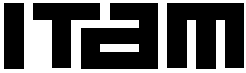
\includegraphics[width=0.55\textwidth]{logoitam}
        
        \vspace{0.8cm}
        \LARGE
        Vector Error-Correction Model
        
        \vspace{1.1cm}
        
        \normalsize \textbf{TESIS}\\ QUE PARA OBTENER EL TÍTULO DE\\ \textbf{LICENCIADO EN MATEMÁTICAS APLICADAS}\\[0.8cm]
        \normalsize \textbf{P\ \  R\ \  E\ \  S\ \  E\ \  N\ \  T\ \  A}\\[0.8cm]

        \textbf{OMAR DÍAZ LANDA}\\[1.0cm]

        \normalsize ASESOR: \textbf{\ \ DR. JUAN JOSÉ FERNÁNDEZ DURÁN}\\[1.0cm]

        \normalsize \textbf{MÉXICO, D.F.} {\ \ \ \ \ \ \ \ \ \ \ \ \ \ \ \ \ \ \ \ \ \ \ \ \ \ \ \ \ \ \ \ \ \ } \textbf{2016}
    \end{center}
\end{titlepage}

\thispagestyle{empty}
\noindent Con fundamento en los artículos 21 y 27 de la Ley Federal del Derecho de Autor y como titular de los derechos moral y patrimonial de la obra titulada ``ANÁLISIS DE COMPONENTES PRINCIPALES BASADO EN KERNELS'', otorgo de manera gratuita y permanente al Instituto Tecnológico Autónomo de México y a la Biblioteca Raúl Bailléres Jr., autorización para que fijen la obra en cualquier medio, incluido el electrónico, y la divulguen entre sus usuarios, profesores, estudiantes o terceras personas, sin que pueda percibir por tal divulgación una contraprestación.\\\\\\\\

\begin{center} 
Itzel Zayil Muñoz Fernández de Córdova\\
\par\noindent\makebox[2.5in]{ }\\
\vspace{10mm}
\par\noindent\makebox[2.5in]{\hrulefill}\\
\par\noindent\makebox[2.5in][c]{Fecha}\\
\par\noindent\makebox[2.5in]{ }\\
\vspace{10mm}
\par\noindent\makebox[2.5in]{\hrulefill}\\
\par\noindent\makebox[2.5in][c]{Firma}\\
%Fecha:\\
%\rule[1em]{25em}{0.5pt} % This prints a line for the signature 
%Firma:\\
%\rule[1em]{25em}{0.5pt} % This prints a line to write the date
%}
\end{center}
\clearpage % Start a new page
 
%\addtocontents{toc}{Agradecmientos}
\begin{center}
{\huge \bfseries Agradecimientos\\}
\end{center}

\vspace{4 mm}

A mis papás Javier y Yazmín, y a mi hermano Yaíro, por su amor incondicional, por ser mi ejemplo a seguir, y por estar a mi lado en cada paso.

\vspace{4 mm}

A mi familia, por su inmenso amor, apoyo, confianza y sabiduría.

\vspace{4 mm}

A Omar por todo su amor y por compartir su vida y proyectos conmigo.

\vspace{4 mm}

A mis amigos, por su cariño, hermandad y por hacerme reír cada día.

\vspace{4 mm}

A mis profesores Rubén Hernández Cid, Fernando Esponda, Ernesto Barrios, y mi colega Luis Díaz, por sus enseñanzas y atención.


\clearpage
\tableofcontents
%\listoffigures

\mainmatter
\chapter{Introducción}
%\input{chapters/chapter01}

\chapter{Teoría de Cointegración}
%\documentclass{article}
%\usepackage[spanish]{babel}
%\usepackage{fullpage}
%\usepackage[pdftex]{graphicx}
%\usepackage{color}
%\usepackage{colortbl}
%\usepackage[usenames,dvipsnames]{xcolor}
%\usepackage{enumerate}
%\usepackage{booktabs}
%\usepackage{amsmath}
%\usepackage{amssymb} %% atencion se agrego un paquete
%\spanishdecimal{.}



%\begin{document}
%\title{Cap\'itulo $2$ tesis}
%\author{Omar D\'iaz Landa\\ Instituto Tecnol\'ogico Aut\'onomo de M\'exico\\ Dr. Juan Jos\'e Fern\'andez Dur\'an}
%\maketitle

%Comentarios: 
%\newpage
\section*{Tero\'ia de Cointegraci\'on}

\subsection{Series de Tiempo}

Es necesario familiarizarse con determinados conceptos de uso frecuente en el an\'alisis de series de tiempo. En la actualidad, es m\'as com\'un el uso del enfoque estoc\'astico que el de descomposici\'on de series, debido a que ha demostrado mayor eficacia en la creaci\'on de modelos y flexibilidad para extenderse a modelos para varias series simult\'aneas.\\

Se dice que es un \textbf{proceso estoc\'astico} si se tiene un conjunto indice lineal\footnote{Sean $t_1$ y $t_2$ $\in$ $T$ entonces $t_1+t_2$ $\in$ $T$} $T$ y  una colecci\'on de variales aleatorias definidas en un espacio de probabilidad tales que para cada variable aleatoria le corresponde un s\'olo elemento del conjunto \'indice, es decir,  $\{Z_t: t \in T\}$. Por lo tanto, una \textbf{serie de tiempo} es un proceso estoc\'astico cuyo conjunto \'indice es el tiempo.\\

Es importante aclarar que cuando se tiene una serie de tiempo observada, contin\'ua siendo un proceso estoc\'astico en el sentido de que cada observaci\'on es una realizaci\'on de una variable aleatoria; consecuentemente una serie de tiempo observada es una realizaci\'on de muchas series posibles.\\

El comportamiento de un proceso estoc\'astico esta descrito completamente por su funci\'on de densidad conjunta, sin embargo, conocerla en el caso de series de tiempo es muy complejo y no es posible obtenerla a partir del producto de las funciones de densidad marginales, ya que las variables son altamente dependientes, en realidad, se trata de la misma variable pero medida en diferentes momentos de tiempo. Debido a lo anterior, el an\'alisis de series de tiempo propone conocer los primeros y segundos momentos, es decir, esperanzas, varianzas y covarianzas para poder caracterizar la serie, pues resumen en buena medida a la funci\'on de densidad conjunta. Adem\'as, nos dar\'an apertura para introducir uno de los conceptos de mayor importancia, el de \textbf{estacionariedad}.\\

Un \textbf{proceso estoc\'astico estrictamente estacionario} es un proceso estoc\'astico cuya distribuci\'on de densidad conjunta es invariante ante desplazamientos en el tiempo, de manera que si se calculan las medias, varianzas y covarianzas, se obtendr\'an los mismos resultados sin importar la longitud y momento de tiempo en que se midan, es decir, las medias y varianzas son constantes en el tiempo y las covarianzas dependen \'unicamente de la distancia entre  los dos periodos de tiempos que se calculan. Cuando no es posible conocer la funci\'on de densidad conjunta y se utiliza los primeros y segundos momentos para determinar estacionariedad se le conoce como \textbf{estacionariedad de segundo orden} o \textbf{estacionariedad d\'ebil}. En resumen, si $Z_t$ es un proceso estacionario tiene las siguientes caracter\'isticas:


\begin{eqnarray}
        Media: & E(Z_t)=\mu   \\ 
        Varianza:  & Var(Z_t)=E[(Z_t- \mu )^2]=\gamma_0   \\ 
        Covarianza & E(Z_t-\mu)E(Z_{t+k}-\mu)=\gamma_k   
\end{eqnarray} 


El concepto de estacionariedad es de suma importancia, ya que los modelos econom\'etricos requieren de series estacionarias para poder analizar el comportamiento de la serie en los periodos observados, generalizarlo a otros periodos de tiempo y ajustar modelos para el pron\'ostico; tal es el caso de los modelos ARIMA de los cuales se hablar\'a m\'as adelante.\\ 

Existen diversas pruebas de estacionariedad, pero en la pr\'actica, las m\'as comunes son el \textbf{an\'alisis gr\'afico} y la \textbf{funci\'on de autocorrelaci\'on}. La primera de ellas es poco confiable, ya que consiste, como su nombre lo indica, en graficar la serie y observar que no muestre tendencias, cambios de nivel o que la viariabilidad aumente con el tiempo, esta prueba sirve para darnos una idea del comportamiento de la serie pero se debe considerar como un paso incial para un an\'alisis m\'as formal como el c\'alculo de la funci\'on de autocorrealci\'on.\\ 

Como mencionamos anteriormente, se deben calcular las medias, varianzas y covarianzas para caracterizar, auqnue no completamente, a una serie de tiempo, sin embargo, al solo tener una realizaci\'on del proceso se debe trabajar con las definciones muestrales:

\begin{eqnarray}
        \mbox{\emph{Media muestral:}} & \bar{Z} =\frac{1}{N} \sum_{t=1}^{N}{Z_t} &   \\ 
        \mbox{\emph{Varianza muestral:}}  & \hat{\gamma_0}=\frac{1}{N} \sum_{t=1}^{N}(Z_t- \bar{Z} )^2 & \\ 
        \mbox{\emph{Covarianza muestral:}} & \hat{\gamma_k}=\frac{1}{N} \sum_{t=1}^{N-k}(Z_t-\bar{Z})(Z_{t+k}-\bar{Z})  & k=0,1,2,... 
\end{eqnarray} 

Con estos t\'erminos es posible obtener la funci\'on de autocorrealci\'on muestral definida como:

\begin{equation}
\hat{\rho_k}= \frac{\hat{\gamma_k}}{\hat{\gamma_0}}=\frac{\sum_{t=1}^{N-k}(Z_t-\bar{Z})(Z_{t+k}-\bar{Z})}{\sum_{t=1}^{N}(Z_t- \bar{Z} )^2}
\end{equation}

Si la funci\'on de autocorrelac\'on tiende r\'apidamente a cero, nos enfrentamos ante un proceso estacionario; si por el contrario, el decaimento de la funci\'on es paulatino, quiere decir que las observaciones del proceso muestran una tendencia que las hace depender de  otras observaciones en el tiempo, provocando que el nivel de la seria se vea afectado por dicha tendencia y existan correlaciones distinstas a cero en periodos de tiempo distantes. Esto \'ultimo nos hace pensar que la serie no cumple con alguna de las caracter\'isticas de un proceso estacionario de segundo orden. \\


Cuando una serie es no estacionaria, s\'olo se puede analizar el periodo observado, no es posible hacer uso de los modelos ARMA y cualquier otro tipo de an\'alisis como por ejemplo una regresi\'on, se debe realizar con particular precauci\'on, ya que se podr\'ia estar en presencia de un fen\'omeno que Yule en 1926\footnote{Yule, G. U., "Why Do We Sometimes Get Nonsense Correlations Between Time Series-' A Study in Sampling and the nature of Time Series", Journal of the Royal Statisticar Society, vol. 89,1926, pp.1-64.} identifica como regresi\'on espurea. Sin embargo, existen herramientas que ayudan a convertir una serie no estacionaria en estacionaria, dichas herramientas son las diferencias estacionarias y diferencias estacionales.\\

Sea el proceso $Z_t$ tal que al aplicar el \textbf{operador difernecia $\nabla$ } se tiene que  $\nabla Z_t=Z_t-Z_{t-1}$. De manera que $\nabla Z_t$ corresponde al cambio en el valor de la variable $Z$ del periodo $t-1$ al periodo $t$, por lo que cuenta con una observaci\'on menos que $Z_t$. Al aplicar el operador la serie obtenida es estacionaria en cuanto a su nivel, pues elimina la tendencia polinomial adaptiva que se encontraba en el proceso. \\

Si la tendencia polinomial adaptiva es de orden mayor a uno se debe considerar aplicar el operador tantas veces como sea necesario, es decir, se existe presencia de una tendencia polinomial de orden $2$, la serie requiere de tomar dos diferencias para estacionarizarla. Ademas, es importante mencionar el riesgo que existe con la sobrediferenciaci\'on pues conlleva a problemas relacionados con la identificaci\'on de un modelo para el proceso, incremento en la varianza y p\'erdida innecesaria de observaciones, pues se pierde una con cada aplicaci\'on del operador.\\

En ocasiones, nos enfrentamos a series que presentan otro tipo de tendencia que se caracteriza por tener un patron de cambio que se repite con una intesidad similar, en determinados periodos de tiempo a\~no con a\~no. Este fen\'omeno es llamado \textbf{estacionalidad} y para controlarlo es necesario en primera instancia identificar el comportamiento peri\'odico de la serie, ya sea que se trate de meses, trimestes, semestres, a�os, periodos vacacionales o cualquier otro hecho que provoque que la serie tenga un comportamiento parecido  en periodos definidos cada a\~no, posteriormente, se hace uso del \textbf{ operador diferencia estacional}  $\nabla_{E}^{k}$  donde $E$ es periodo que contiene la tendencia-ciclo y $k$ es el n\'umero de veces necesarias que se debe aplicar el operador diferencia para hacer la serie estacionaria.\\

El operador diferencia estacional esta definido de la siguiente manera:

\begin{equation}
\nabla_{E}=Z_t-Z_{t-E}
\end{equation}

Al igual que en el operador diferencia estacionaria $\nabla$ se pierden observaciones cada vez que se aplica, en este caso se trata de $E$ observaciones.\\

Cuando a un proceso es necesario aplicarle el operador diferencia $\nabla$  una vez para hacerlo estacionario, se dice que es un proceso integrado de orden $1$ y se denota $Z_t \sim I(1)$. De manera similar, si se requieren $2$ diferencias para estacionarizar la serie se trata de un proceso integrado de orden dos y si necesitamos $d$ diferencias es un proceso integrado de orden d,  $Z_t \sim I(d)$, finalmente, si $z_t$ es estacionario nos podemos referir a este proceso como un proceso estacionario o como un proceso intregrado de orden cero. En general, el orden de integraci\'on depende del m\'inimo n\'umero de difrencias que se deben aplicar al proceso para convertirlo en estacionario. Este concepto de procesos estoc\'asticos integrados trae consigo las siguientes propiedades:\\

Sean $Z_t$, $Y_t$ y $W_t$ tres procesos estoc\'asticos

\begin{enumerate}%for small alpha-characters within brackets.

\item
 Si $Z_t \sim I(0)$ y  $Y_t \sim I(1)$ entonces $W_t=(Z_t+Y_t) = I(1)$ es decir, una combinaci\'on lineal entre un proceso estacionario y uno no estacionario es no estacionario.

\item
Si $Z_t \sim I(d)$ etonces $W_t=(a+bZ_t)=I(d)$, donde $a$ y $b$ son constantes. Una combinaci\'on lineal de un proceso no estacionario, es no estacionario. Por lo tanto, la combianci\'on lineal de un proceo estacionario contin\'ua siendo estacionario.

\item 
Si $Z_t \sim I(d_1)$ y $Y_t \sim I(d_2)$ entonces $W_t=(aZ_t+bY_t)=I(d_2)$ ya que $d_1<d_2$.

\item
Si $Z_t \sim I(d)$  y $Y_t \sim I(d)$ entonces $W_t=(aZ_t+bY_t)=I(d^*)$ donde $d^*$ generalmente es igual a $d$, aunque en ocasiones $d^* < d$. 

\end{enumerate}

Como es posible observar, trabajar con varias series que no tienen el mismo orden de integraci\'on puede resultar complicado. Sin embargo, en el siguiente cap\'itulo se presentar\'an t\'ecnicas apropiadas para reducir estos riesgos. 



%%%%%%%%%%%%%%%%%%%%%%%%%%%%%%%%%%%%%%%%%%%%%%%%%%%%%%%%%%%%%%Raiz unitaria
\subsection{Ra\'iz Unitaria: Pruebas}

Consideremos el siguiente proceso determinista:
\begin{eqnarray}
Z_t = a_0+a_1 Z_{t-1} &  t=...,-2,-1,0,1,2,...
\end{eqnarray}

que tambien puede ser expresado a partir del uso del operador $L$ que proviene del ingl\'es $Lag$ y se define como $LZ_t=Z_{t-1}$, por lo tanto $ Z_t = a_0+a_1 Z_{t-1}$ ahora es
\begin{eqnarray}
(1-a_1L)Z_t = a_0,  & &  t=...,-2,-1,0,1,2,...
\end{eqnarray}

si se despeja a $Z_t$ del proceso tendr\'iamos la siguiente operaci\'on, que al desarrollarla se sigue que 

\begin{eqnarray}
 (1-a_1L)^{-1} a_0 =&  \sum_{i=0}^{\infty} (a_1L)^{i}a_0  &  \nonumber  \\ 
        = & a_0\sum_{i=0}^{\infty} (a_1L)^{i} & L^i 1=1  \nonumber \\
         = & a_0\sum_{i=0}^{\infty} (a_1)^{i} &  \\
         = & \frac{a_0}{1-a_1} & \left | a_1 \right |<1  \nonumber \\
 & &  \nonumber
\end{eqnarray}


En la expresi\'on anterior, el supuesto $\left | a_1 \right |<1$ permite la convergencia de la serie geom\'etrica real, sin embargo, $a_1$  puede tomar cualquier valor excepto $a_1=1$.   Por lo tanto, la soluci\'on general para este proceso ser\'ia de la forma 

\begin{equation}
Z_t=\frac{a_0}{1-a_1} + sa_1^t
\end{equation} 

donde  el t\'ermino $sa_1^t$ se agrega para poder brindar soluciones particulares a partir de la constante $s$. Ahora bien, si por un lado conservamos el supuesto de la expresi\'on $(11)$, es decir, que la ra\'iz de la ecuaci\'on $(1-a_1L)=0$ cumpla que $\left | a_1 \right |<1$  podemos observar que

\begin{equation}
\lim_{t\rightarrow \infty } Z_t=\frac{a_0}{1-a_1}
\end{equation}   

lo cual  indica que el proceso determinista alcanzar\'a un punto de equilibrio en el largo plazo. Por otro lado, si $a_1=1$ entonces el proceso diverge, ya que el cociente $\frac{a_0}{1-a_1}$ quedar\'ia indeterminado y si  $\left | a_1 \right |>1$ el proceso no converge y por lo tanto jam\'as tender\'a a estabilizarse.\\

Ahora que se entiende la problem\'atica que existe cuando se tienen raices unitarias en procesos deterministas, es oportuno llevar estos resultados a procesos estoc\'asticos, de manera que si definimos a la constante $a_1=1$, la constante $a_0=(1-L)Z_0$ y agregamos una variable aleatoria que depende del tiempo $e_t$\footnote{ Mejor conocida como ruido blanco} con media cero, varianza constante $\sigma_e^2$y no correlacionada, tendr\'iamos al siguiente proceso:

\begin{equation}
Z_t= Z_{t-1} + a_0 + e_t
\end{equation} 

que a su vez puede ser reexpresada como

\begin{eqnarray}
(1-L)Z_t =& a_0 + e_t & \nonumber \\
(1-L)Z_t =& (1-L)Z_0 + e_t & \nonumber \\
(1-L)\tilde{Z}_t =& e_t & \mbox{con $\tilde{Z}_t =Z_t-Z_0$}
\end{eqnarray}
\label{eq:AR1}  

Este proceso contiene el valor obtenido en el periodo pasado mas un error en cada una de las realizaciones, de manera que cada realizaci\'on de la variable aleatoria ${e_t}$ en cada momento $t$ proporciona una tendencia estoc\'astica que provoca que el proceso tenga fluctuaciones, por lo tanto, no es correcto decir que el proceso alcance un punto de equilibrio, sino que se tendr\'a que recurrir al concepto de estacionariedad ya conocido. En este particular caso, las fluctuaciones implicar\'ian que si tomamos medias muestrales en diferentes intervalos de tiempo, obtendr\'iamos diferentes resultados, caractar\'istica  que nos indica que la serie es no estacionaria. Para comprobar lo anteriormente mencionado, calculamos los dos primeros momentos del proceso despu\'es de haber inferido el comportamiento de la serie con el m\'etodo iterativo.

 \begin{eqnarray}
 E(\tilde{Z}_t) &  =&   E(e_1+ e_2+...+e_t)= 0 \nonumber  \\ 
         &  &    \\
         Var(\tilde{Z}_t) & =& Var(e_1+e_2+...+e_t)=t \sigma_e^2  \nonumber \\
 & &  \nonumber 
\end{eqnarray} 


Por lo que podemos observar que no cumple con los supuestos que requiere la estacionariedad de segundo orden, pues la varianza aumenta conforme se avanza en el tiempo causando que el proceso no regrese a su nivel esperado. Por el contrario, si el valor de la constante $a_1$ es menor que la unidad, entonces el proceso es estacionario y se demuestra calculando nuevamente los momentos de primer y segundo orden, para facilitar la operaci\'on reexpresamos al proceso usando la serie geometrica de la siguiente manera:

\begin{equation}
\tilde{Z}_t=(1-a_1L)^{-1}e_t=e_t+a_1e_{t-1}+a_1^2e_{t-2}+ a_1^3e_{t-3}+...
\end{equation} 

Por lo tanto, la media y la varianza del proceo son

 \begin{eqnarray}
 E(\tilde{Z}_t) &  =&  E(e_t) + a_1E(e_{t-1})+ a_1^2E(e_{t-2})+...= 0 \nonumber  \\ 
         &  &    \\
         Var(\tilde{Z}_t) & =& \sigma^2_e (1+a_1^2+ a_1^4+ ...)= \frac{\sigma_e^2}{(1-a_1^2)}  \nonumber \\
 & &  \nonumber 
\end{eqnarray}

Que demuestran estacionariedad de segundo orden ya que ninguna depende del tiempo. Por lo anterior, es de nuestro inter\'es hacer pruebas sobre el valor de $a_1$ para determinar si es estad\'isticamente igual a la unidad, por lo tanto, en la prueba de hipotiesis correspondiente, se tendr\'ia como hip\'otesis nula el hecho de que $a_1=1$ que implicar\'ia no estacionariedad en el proceso, mientras que la hip\'otesis alternativa abarca los posibles valores de $a_1$ que proporcionan un proceso estable:

   \begin{eqnarray}
    H_0: a_1=1 &  &  H_a:\left | a_1 \right |<1   \\ 
    \nonumber 
   \end{eqnarray} 

No obstante es posible reparametrizar al proceso sustrayendo en cada lado de la ecuaci\'on el valor $Z_{t-1}$, con la finalidad de que la prueba sea similar a la prueba sobre coeficientes individuales de regresi\'on


 \begin{eqnarray}
 Z_t-Z_{t-1} &  =& a_1Z_{t-1}-Z_{t-1}+e_t\nonumber  \\ 
       \nabla Z_t &= & (a_1-1)Z_{t-1}+e_t   \\
         \nabla Z_t & =& \rho Z_{t-1}+e_t  \nonumber \\
 & &  \nonumber 
\end{eqnarray}

donde $\rho=(a_1-1)$ de manera que la nueva hip\'otesis nula y alternativa son:

   \begin{eqnarray}
    H_0: \rho=0 &  &  H_a:\left | \rho \right |<1   \\ 
    \nonumber 
   \end{eqnarray} 


 As\'i que $\rho=0$ implica que $a_1=1$ trat\'andose de un proceso no estacionario, mientras que si se rechaza la hip\'otesis nula tendremos un proceso estable, la parte $\left | \rho \right |>1$ no se considera pues la serie ser\'ia explosiva. Esta \'ultima prueba es la llamada \textbf{Prueba de Dickey-Fuller} y es cumplemento formal a los m\'etodos ya mencionados como la gr\'afica de los valores de la serie respecto al tiempo, el uso del autocorrelograma y la varianza muestral para determinar estacionariedad, as\'i como el n\'umero de diferencias necesarias para convertir la serie en estacionaria.\\
 
 Para hacer uso de la prueba, es imprescindible conocer el valor del coeficiente $\rho$ pero como se dijo anteriormente, la prueba es en esencia la misma que para los coeficientes de una regresi\'on, as\'i que se estima este valor por medio de m\'inimos cuadrados. Si $\rho >0$ implica que $a_1>1$ por lo que se puede concluir r\'apidamente que la serie es no estacionaria, no obstante, si $\rho \leq 0$ se tiene que observar si es estad\'isticamente diferente de cero, as\'i que se calcula el estad\'istico de prueba
 
 \begin{equation}
 \tau_0=\frac{\hat{\rho}}{se(\hat{\rho})}
 \end{equation}
 
Si el proceso es estacionario, se puede continuar con el an\'alisis usual de las pruebas sobre coeficientes individuales de una regresi\'on, sin embargo, cuando el proceso no lo es, se tiene la particularidad de que no se distribuye como una $t-Student$, ya que si se aceptara la hip\'otesis nula, $Z_t$ ser\'ia un proceso no estacionario cuya varianza aumenta conforme se incrementa el tama\~no de muestra, provocando que la distribuci\'on usual $t-Student$ se modifique. La contribuci\'on de Dickey y Fuller consisti\'o en la creaci\'on de los valores cr\'iticos del estad\'istico $\tau$ para tres diferentes procesos  a partir de simulaciones de Monte Carlo. Dichos procesos corresponden en primer lugar, al mostrado en la ecuaci\'on $(19)$. \\

En segundo lugar, al proceso

 \begin{equation}
 \nabla Z_t= \alpha +  \rho Z_{t-1}+e_t
 \end{equation}
 
donde cada realizaci\'on de la variable $\nabla Z_t$ depende del valor de una constante, m\'as una proporci\'on del valor anterior $Z_{t-1}$, m\'as el error $e_t$. Estos procesos comunmente presentan tendencias definidas hacia arriba si el valor de $\alpha$ es positivo y tendencias definidas decrecientes si es negativo, es decir, tienen una tendencia determin\'istica, ya que se le agrega un valor constante $\alpha$ en cada instante de tiempo $t$. En este caso, si rechazamos la hip\'otesis nula, es posible hablar de un proceso estacionario pero con media distinta de cero.\\

Finalmente, tenemos al proceso que incluye constante y una tendencia en el tiempo

 \begin{equation}
 \nabla Z_t= \alpha + \beta t + \rho Z_{t-1}+e_t
 \end{equation}
 
como es posible observar, el nuevo t\'ermino proporciona impacto a la tendencia en cada instante de tiempo, si la prueba de hip\'otesis refleja que el coeficiente $\rho \neq 0$ entonces se trata de un proceso estacionario al rededor de una tendencia determin\'istica. Para los tres casos se usa la misma prueba de hip\'otesis y  el mismo estad\'istico de prueba pero diferentes valores cr\'iticos que dependen del tama\~no de la muestra, tal y como se muestra en la siguiente tabla. El estad\'istico $\tau$ debe ser m\'as negativo que el valor cr\'itico correspondiente para rechazar la hip\'otesis nula $(\tau \leq \tau^*)$.\\


\begin{table}[ht]
\caption{\textbf{Valores Cr\'iticos para la prueba Dickey-Fuller}}
\centering
   \begin{tabular}{lccc}
\arrayrulecolor{RoyalBlue}\toprule
    $Model$                                               &  $1\%$    &  $5\%$    & $10\%$   \\
\arrayrulecolor{Cerulean}\hline
    $\nabla Z_t =\rho Z_{t-1} + e_t$                     &  $-2.56$ & $-1.94$ & $-1.62$ \\
    $\nabla Z_t = \alpha + \rho Z_{t-1} + e_t$            &  $-3.43$ & $-2.86$ & $-2.57$ \\
    $\nabla Z_t = \alpha + \beta_1 t + \rho Z_{t-1} + e_t$ & $-3.96$ & $-3.41$ & $-3.13$ \\
\arrayrulecolor{Cerulean}\hline
    $Standard$  $critical$ $values$                         & $-2.33$ & $-1.65$ & $-1.28$ \\
\arrayrulecolor{Cerulean}\hline
    \end{tabular}
\end{table}
\label{table:CVDF}







Tiempo despu\'es, los supuestos de la prueba de Dickey-Fuller se vieron relajados permitiendo que existiera correlaci\'on entre los errores, la cual puede surgir cuando el modelo no captura la din\'amica completa del proceso, es decir, le faltan elementos para explicar a la variable. Lo anterior se corrige agregando un mayor n\'umero de diferencias de primer orden, tantas como sean necesarias para asegurar que la correlaci\'on en los residuos desaparezca, estas  se pueden determinar con el gr\'afico de las autocorrelaciones considerando todas aquellas que sean grandes y descartando de manera formal las que no son necesarias con la significancia de los coeficientes  $\beta_i$, obteniendo as\'i el siguiente proceso general:

  \begin{equation}
 \nabla Z_t= \alpha + \beta_1 t + \rho Z_{t-1} + \sum_{i=1}^{m} \beta_i \nabla Z_{t-i} + e_t
 \end{equation}


Analogamente a la prueba no aumentada, se debe procourar no incluir o excluir el t\'ermino constante y a la tendencia determin\'istica cuando no es necesario, ya que podr\'ia traer problemas de sesgo al estad\'istico $\tau$ y p\'erdida de significancia de la prueba si se eligen err\'oneamente los valores cr\'iticos, es posible hacer uso de los mismos valores mostrados en el cuadro ~\ref{table:CVDF} \textcolor{red}{ num tabla }, ya que la prueba de Dickey-Fuller aumentada sigue la misma distribuci\'on asint\'otica.  


  \subsection{Modelos para series de tiempo univariadas}

La metodolog\'ia propuesta por Box y Jenkins se convirti\'o en una herramienta muy popular para el an\'alisis de series de tiempo,  cuya principal funci\'on era el pron\'ostico de valores futuros y  modelar los valores observados de una serie de tiempo. Estos modelos son conocidos como \textbf{autoregresivos e integrados de promedios moviles}, ya que est\'an formados por una parte autoregresiva considerando $p$ retrasos, una parte de $q$ choques aleatorios en el tiempo y, si es necesario, las $d$ diferencias que indique el orden de integraci\'on para que el procceso sea estacionario en cuanto a su nivel; de manera que lo anterior usualmente es referido como $ARIMA(p,d,q)$. 

\subsubsection{Modelos Autoregresivos}

Como su nombre lo indica, se trata de una regresi\'on lineal con la diferencia de que las variables independientes, en este caso, son retrasos de la variable dependiente, es decir,  la variable se explica a partir de la historia de sus valores pasados. El caso m\'as simple, es el que encontramos en la ecuaci\'on  (\ref{eq:AR1}) \textcolor{red}{ num equ 14} denominado como autoregresivo de orden 1 $AR(1)$, ya que s\'olo es explicado por una proporci\'on de su valor retrasado un periodo m\'as el efecto que brinda el ruido blanco.

  \begin{equation}
  \tilde{Z}_t= \phi \tilde{Z}_{t-1} + e_t
 \end{equation}

Es necesario recordar que para tener una serie estacionaria el valor de $\phi$ debe ser menor a la unidad en valor absoluto y que la media y la varianza est\'an dados por:

\begin{eqnarray}
E(\tilde{Z}_t)&=&0\\
Var(\tilde{Z}_t)&=& \frac{\sigma_e^2}{1-\phi^2}
\end{eqnarray} 


As\'i que la varianza de la serie de tiempo autoregresiva de orden uno depende del valor de la constante $\phi$ y de la varianza de $e_t$; para el c\'alculo de las autocovarianzas entre dos series $Z$ que se encuentran separadas por un periodo tenemos que

\begin{eqnarray}
Cov(\tilde{Z}_t,\tilde{Z}_{t-1})&=& E\left [ \tilde{Z}_t \tilde{Z}_{t-1} \right ] \nonumber \\
&=& E\left [ (e_t+\phi e_{t-1} + \phi^2 e_{t-2}+\phi^3  e_{t-3} + \cdots )(e_{t-1}+\phi e_{t-2} + \phi^2 e_{t-3}+\phi^3  e_{t-4} + \cdots )\right ] \nonumber \\
&=& \phi E(e_{t-1}^2)+ \phi^3 E(e_{t-2}^2) + \phi^5 E(e_{t-3}^2)+ \cdots \nonumber \\
&=& \phi \sigma_e^2( 1 + \phi^2 +\phi^4 + \cdots) \nonumber \\
Cov(\tilde{Z}_t,\tilde{Z}_{t-1})&=& \frac{\phi \sigma_e^2}{1-\phi^2}
\end{eqnarray} 

por lo tanto, el autocorrelograma obtiene sus valores mediante la divisi\'on de las autocovarianzas entre la varianza de la serie de tiempo, esto es

\begin{equation}
\rho_k=\frac{Cov(\tilde{Z}_t,\tilde{Z}_{t-1})}{Var(\tilde{Z}_t)}=\phi^{\left | k \right |}  \hspace{15mm}  k=\pm0, \pm1 ,\pm2,...
\end{equation} 

de manera que la correlaci\'on entre errores que se encuentran $k$ periodos separados, es el valor de $\phi$ elevado a la $k-esima$ potencia. El autocorrelograma tender\'a a mostrar comportamientos diferentes dependiendo de los valores que tomen las raices del polinomio caracter\'istico de la serie de tiempo, es decir, si las raices son positivas y menores que uno, el decaimiento sera exponencial, por el contrario, si son negativas y mayores a $-1$ el decaimiento ser\'a alternadamente. El panorama deseado consiste en que el decaimineto del autocorrelograma tienda a cero de manera exponencial, lo cual se ver\'a favorecido mientras se incrementa el valor de $k$, sin embargo, en ocasiones algunas correlaciones resultan ser significativamente diferentes de cero, lo que nos lleva a pensar que nuestro modelo autoregresivo de orden 1 no captura en buena medida la din\'amica del proceso y por lo tanto es necesario introducir una mayor cantidad de retrasos, por ejemplo $p$. A esto se le conoce como modelo autoregresivo de orden $p$, $AR(p)$, as\'i que el orden del modelo es igual al restraso m\'as largo de la serie $Z$.

\begin{equation}
\tilde{Z}_t= \theta_1 \tilde{Z}_{t-1} + \theta_2 \tilde{Z}_{t-2} + \theta_3 \tilde{Z}_{t-3} + \cdots + \theta_p \tilde{Z}_{t-p} + e_t
\end{equation} 


al igual que en el caso anterior, es posible determinar la funci\'on de autocorrelaci\'on en func\'on de los coeficientes autoregresivos del modelo $AR(p)$, que deber\'a mostrar un decaimiento exponencial a cero cuando las raices del polinomio caracter\'istico asociado a la serie se encuentren fuera del c\'irculo unitario, es decir, es estacionario. \\

Una caracter\'istica que poseen todos los modelos autorregrisvos conocida como invertibilidad consiste en poder ser represantados, como se puede observar en la ecuaci\'on   \textcolor{red}{ num tabla  $17$}, como una suma infinita ponderada de choques aleatorios:

\begin{equation}
\tilde{Z}_t= e_t  + \psi_1 e_{t-1} + \psi_2 e_{t-2} +\psi_3 e_{t-3} +  \cdots  \hspace{15mm} \mbox{\emph{con}}  \hspace{9mm} \sum_{i=1}^{\infty } \left | \psi_i \right | < \infty 
\end{equation} 

\'Esta expresi\'on explica exactamente lo mismo que la representaci\'on con par\'ametros finitos, por lo que es recomendable trabajar con \'esta \'ultima. Sin embargo, se da apertura para pensar que existan fen\'omenos econ\'omicos, financieros o incluso naturales que puedan ser modelados a partir de choques aleatorios ponderados, los cuales son conocidos en el an\'alisis de series de tiempo como \textbf{Modelos de Promedios M\'oviles}.


\subsubsection{Modelos Promedios M\'oviles}

Es posible hallar otros mecanismos que pudieron haber generado al proceso estoc\'astico $Z_t$ como por ejemplo, a partir de una combinaci\'on lineal de los t\'erminos del error a lo largo del tiempo, es decir, como una suma finita ponderada de choques aleatorios independientes.

 \begin{equation}
\tilde{Z}_t= \theta (L)e_t=(1-\theta_1L-\theta_2L^2 - \cdots -\theta_qL^q)e_t=  e_t  + \theta_1 e_{t-1} + \theta_2 e_{t-2}  +  \cdots +\theta_q e_{t-q}  
\end{equation} 
  
Donde $\tilde{Z}_t$ son las desviaciones de $Z_t$ respecto a su nivel medio $\mu$ y $\theta_i$ para $i=1,2,\cdots,q$ son las ponderaciones asociadas a los choques aleatorios independientes. Esto quiere decir que dado un proceso que se encuentra en equilibrio, presenta fluctuaciones causadas por los choques aleatorios los cuales no necesariamente deben volver al nivel de la serie en el periodo inmediato posterior sino que esto suceder\'a \'unicamente en el largo plazo, adem\'as la intensidad reflejada en cada uno de los t\'erminos del ruido blanco es causada por el valor del coeficiente $\theta_i$ correspondiente. Es natural el querer asociar dichas fluctuaciones independientes con eventos fortuitos que provocan que la serie se aleje de su nivel medio aunque sea moment\'aneamente. La funci\'on que ocupa el t\'ermino de ruido blanco $e_t$ difiere en cada uno de los modelos que hemos visto hasta ahora, ya que un solo impacto de choque aleatorio en el modelo de promedios m\'oviles $MA(q)$ afecta al proceso estoc\'astico $Z$ en el periodo actual y a lo m\'as en $q$ periodos futuros, mientras que en un modelo autoregresivo $AR(p)$ influye infinitamente en los valores futuros, pues el t\'ermino $e_t$ se encuentra en el proceso $Z_t$, $Z_{t+1}$, $Z_{t+2}$ y as\'i sucesivamente.\\

Es menester presentar una de las caracter\'isticas de mayor importancia del modelo de promedios m\'oviles, para ello debemos recordar la representaci\'on de los modelos $AR(p)$ como suma infinita ponderada de choques aleatorios de la ecuaci\'on \textcolor{red}{  17}, la cual tiene como restricci\'on que $\sum_{i=1}^{\infty } \left | \psi_i \right | < \infty$ para poder conocer los primeros momentos del proceso, sin embargo, todo modelo $MA$ satisface dicha condici\'on y si calculamos la media, varianza y covarianzas del modelo $MA(1)$ podemos observar lo siguiente:

El proceso $MA(1)$ es de la forma
 \begin{equation}
\tilde{Z}_t=(1-\theta_1L)e_t=  e_t  + \theta_1 e_{t-1} 
\end{equation} 

A partir del cual se puede conocer su media y su varianza de manera inmediata

 \begin{equation}
E(\tilde{Z}_t)=E( e_t  + \theta_1 e_{t-1})=E(e_t)+\theta_1 E( e_{t-1})=0
\end{equation} 
 
\begin{eqnarray}
Var(\tilde{Z}_t)&=&Var(e_t-\theta_1 e_{t-1}) \nonumber \\
&=& Var(e_t)+Var(\theta_1 e_{t-1}) \nonumber\\
&=& \sigma_e^2 + \theta_1^2 \sigma_e^2\\
&=& \sigma_e^2(1+ \theta_1^2)\nonumber
\end{eqnarray} 

Para el caso de las autocovarianzas se tiene que

\begin{equation}
E[\tilde{Z}_t \tilde{Z}_{t-k}]=E[(e_t-\theta_1 e_{t-1})(e_{t-k}-\theta_1 e_{t-k-1})]= \left\{ \begin{array}{rl}
 -\theta_1 \sigma_e^2 &\mbox{ si $k=1$} \\
  0 &\mbox{si  $k\geq 2$}
       \end{array} \right.
\end{equation}

Por lo que debemos notar que ninguno de sus momentos depende del tiempo, resultado que se puede extener f\'acilmente a modelos de promedios m\'oviles de ordenes mayores a 1. Por lo tanto, es posible identificar como caracter\'istica principal de los Modelos $MA$ que todos son estacionarios. \\

Finalmente, la funci\'on de autocorrelaci\'on es de la forma

\begin{equation}
\rho_k= \left\{ \begin{array}{rl}
 -\frac{\theta_1}{1+ \sigma_e^2} &\mbox{ si $k=1$} \\
  0 &\mbox{si  $k\geq 2$}
       \end{array} \right.
\end{equation}
 
  Al observar la $FAC$ podemos observar que s\'olo la primera autocorrelaci\'on es diferente de cero y las siguientes son todas iguales a cero, de manera que cumplen con el decaimiento exponencial r\'apido de procesos estacionarios, adem\'as indica que el proceso solo recuerda un periodo anterior, es decir, no tiene memoria. Un valor cercano a uno en la primera autocorrelaci\'on puede implicar una fuerte dependencia entre el periodo actual y el periodo anterior, por lo que ser\'ia conveniente proponer un modelo autoregresivo ya que podr\'a captar en mejor medida la din\'amica del proceso, por consiguiente es deseable tener una primera autocorrelaci\'on peque\~na. De igual manera, si se tiene un modelo $MA(q)$ se tendr\'an las primeras $q$ autocorrelaciones diferentes de cero y el resto iguales a cero, donde las primeras $q$ deber\'an ser cortas. 

\subsubsection{Modelos Autoregresivos e Integrados de Promedios M\'oviles}

En la pr\'actica la mayor\'ia de las veces nos enfrentamos con series que no son estacionarias, es decir, que sus primeros momentos no son invariantes en el tiempo. Ya hemos visto que cuando se tienen procesos no estacionarios en cuanto a su nivel es ocasionado, en el agunos casos, por la presencia de una tendencia polinomial adaptiva la cual es posible eliminar mediante la aplicaci\'on del operador diferencia un n\'umero adecuado de veces, sin embargo, cuando la no estacionaridad es provocada por  varianza no constante se debe pensar, como en la regresi\'on lineal m\'ultiple, en una transformaci\'on estabilizadora de varianza. Adem\'as, usualmente los procesos presentan caracter\'isticas tanto de modelos $AR$ como de $MA$ permitiendo as\'i una generalizaci\'on que mezcla a los dos modelos anteriores con el concepto de integraci\'on.

El modelo $ARIMA(p,d,q)$  es el siguiente:

\begin{equation}
\phi(L)\nabla^d\tilde{Z}_t=\theta(L)e_t  \hspace{9mm} d \geq 1
\end{equation} 

donde $\phi(L)$ representa un polinomio de restraso de orden $p$ con par\'ametros autoregresivos, $\theta(L)$ un polinomio de restraso de orden $q$ con par\'ametros de promedios m\'oviles y $\tilde{Z}_t$ un proceso con orden de integraci\'on $d$. Es necesaria esta transformaci\'on en la variable $\tilde{Z}_t$ ya que los modelos $AR$ y $MA$ s\'olo pueden operar con procesos estacionarios, ya que de lo contrario no ser\'ia posible captar de manera correcta la din\'amica del proceso y mucho menos pronosticar para volores futuros. Por lo tanto, al aplicar las $d$ diferencias a un proceso con orden de integraci\'on $d$ se convierte estacionario en cuanto a su nivel permitiendo ser respresentado por una parte autoregresiva y una parte de promedios m\'oviles. El motivo principal de incluir a los dos modelos consiste en utilizar el menor  n\'umero de par\'ametros para describir el comportamiento de la serie considerando tanto los valores del proceso en el pasado como las fluctuaciones provocadas por choques aleatorios. \\

El modelo  $ARIMA(p,d,q)$ no hereda de manera inmediata las caracter\'isticas principales de cada una de sus partes, es decir, no hereda la invertibilidad ni estacionariedad del modelo $AR$ y $MA$ respectivamente. Sin embargo, es factible obtener dichas caracter\'isticas siempre y cuando las raices de los polinomios $\phi(L)$ y  $\theta(L)$ se encuentren fuera del circulo unitario. 









%\end{document}

\chapter{Métodos kernel}
%\input{chapters/chapter03}

\chapter{Análisis de Componentes Principales basado en kernels}
\chaptermark{ACP basado en Kernels}
%\input{chapters/chapter04}

%\chapter{Aplicaciones}
%\input{chapters/chapter05}

\chapter{Conclusiones}
%\input{chapters/chapter06}

%%%%%%%%%%%%%% Apendices %%%%%%%%%%%%%%%
\appendix
\chapter{Conceptos}
%\input{chapters/appendix0}
\chapter{Código}
%\input{chapters/appendix}
%%%%%%%%%%%%%%%%%%%%%%%%%%%%%%%%%%%%%%%%%

%%%%%%%%%%%% Bibliography %%%%%%%%%%%%%%% 
\phantomsection
\clearpage
\addcontentsline{toc}{chapter}{Bibliografía}
\nocite{*}
\bibliography{ref}	
%%%%%%%%%%%%%%%%%%%%%%%%%%%%%%%%%%%%%%%%%

\end{document}